\documentclass{article}

\usepackage{graphicx}
\usepackage{hyperref}
\usepackage{tikz}
\usepackage{pgfplots}
\usepackage{siunitx}


\author{Chirvasa Matei \& Rotariu George}
\title{Homework 0}

\begin{document}
\maketitle

\section{Introduction}
In this homework, we tackle the challenge of determining the global minimum of a multivariable function, on a small range, using a determinstic and a heuristic method.
\subsection{Motivation}
The motivation of this homework is to prove that certain computational problems are too resource-intensive to generate a correct response using a deterministic method, as well as show the consequences of using heuristic methods.

\section{Method}
\subsection{Functions}
For this demonstration we will use Rastrigin's Function\cite{Rastrigin}, Michalewicz's Function\cite{Michalwicz}, the Sum Square Function\cite{SumSquare}, and the Sphere Function\cite{Sphere}
\\Rastrigin's Function:
$$ f(x) = A \cdot n + \sum_{i=1}^n \left[ x_i^2 - A \cdot cos(2 \pi x_i) \right],
A = 10, x_i \in \left[ -1, 1 \right]$$

\begin{figure}[!ht]
  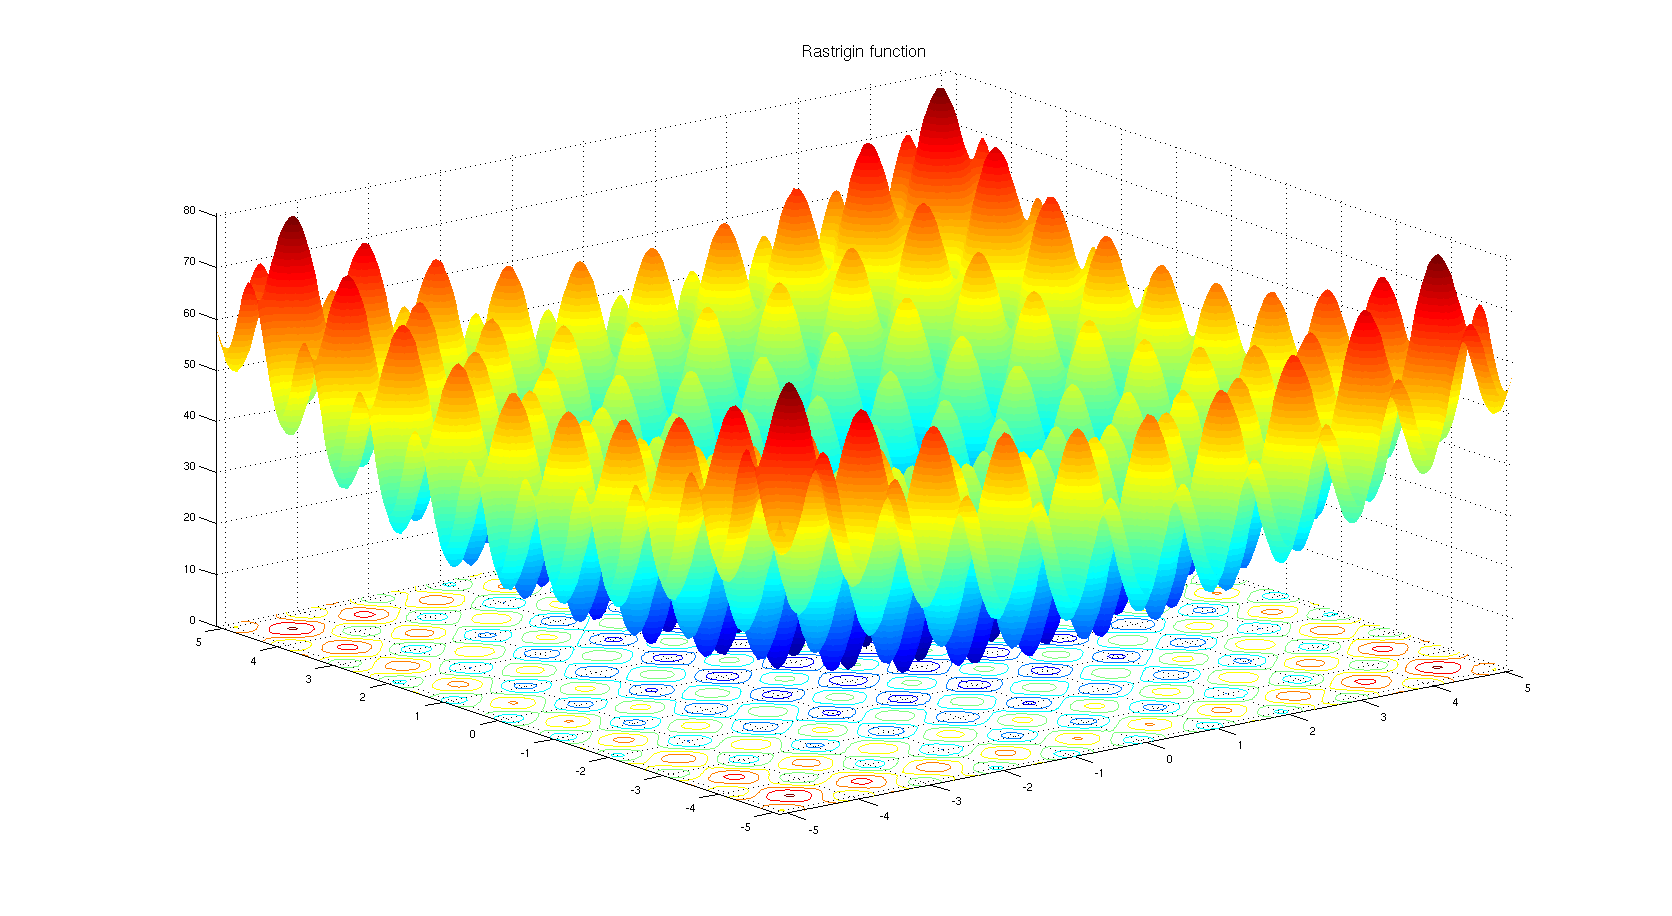
\includegraphics[width=\textwidth,height=\textheight,keepaspectratio]{Rastrigin_function}
  \caption{Rastrigin's Function.}
\end{figure}

Michalewicz's Function:
$$ f(x) = - \sum_{i=1}^n sin(x_i) \cdot sin^{2m}\left(\frac{i \cdot x_i^2}{\pi}\right),
m = 10, x_i \in \left[ 1, 3 \right]$$
\begin{figure}[!ht]
  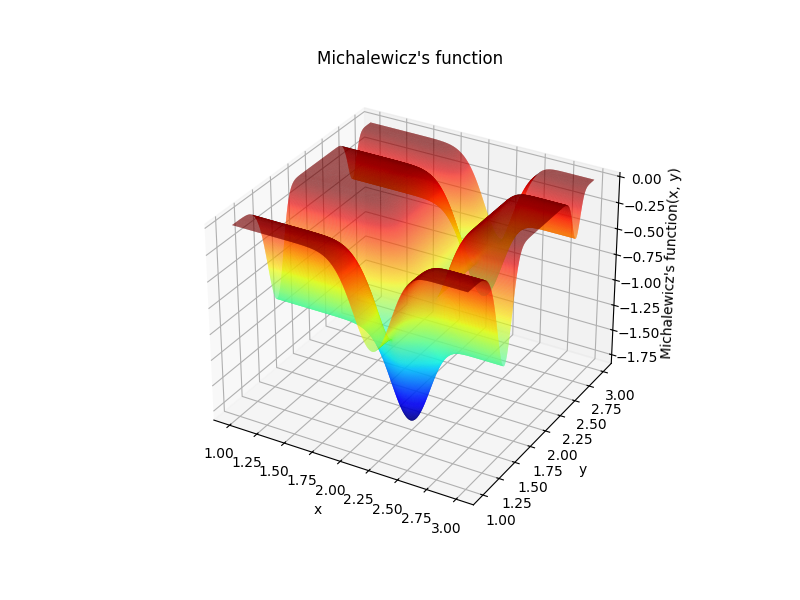
\includegraphics[width=\textwidth,height=\textheight,keepaspectratio]{Michalewicz_function}
  \caption{Michalewicz's Function}
\end{figure}

Sum Square Function:
$$ f(x) = \sum_{i = 1}^n i \cdot x_i^2, x_i \in \left[ -1, 1 \right]$$
\begin{figure}[!ht]
  \includegraphics[width=\textwidth,height=\textheight,keepaspectratio]{}
  \caption{Sum Square Function}
\end{figure}

Sphere Function:
$$ f(x) = \sum_{i = 1}^n x_i^2, x_i \in \left[ -1, 1 \right]$$
\begin{figure}[!ht]
  \includegraphics[width=\textwidth,height=\textheight,keepaspectratio]{}
  \caption{Sphere Function}
\end{figure}

\subsection{Algorithms}
For simplicity, algorithms will be ran with 2 and 10 dimensions.
\\For the determinstic method, we will use a simple algorithm that will generate every possible input $x = (x_1, x_2)$ or $(x_1, x_2, ..., x_9, x_{10})$, with a minimum $x_i$ step of $\varepsilon = \num{e-5}$ . Such an algorithm finds itself in the following complexity class:
$$O\left(\left(\frac{range}{\varepsilon}\right)^d\right), d = \text{Number of dimensions}$$
$$range = \text{Supremum} - \text{Infimum of the function's domain} $$

The algorithm will simply determine $f(x), \forall. x$ where $x_i$ $\in \left[ \text{infimum}, \text{supremum} \right]$.
\\As we know, exponential complexity algorithms are incredibly taxing on computers, and the estimated time required to run the algorithm multiple times may be too big for some time-sensitive tasks. 

The heuristic method will use an algorithm that will generate a random input $x$, and then search for the neighbour that yields the lowest result when the function is applied to it. If no neighbour gives a lower result than that of the current $x$, the algorithm stops, and assumes $x$ is the global minimum of the function. In truth, this algorithm produces a local minimum, chosen at random.
The complexity of such an algorithm is hard to estimate, as it depends on the amount of neighbours the current minimal point must pass through before finding a local minimum. However, we can estimate the amount of steps required to find the lowest neighbour of the current minimal point.
$$ O\left(3^d\right), d = \text{Number of dimensions} $$

This algorithm is also exponential, but given that $d \in \{2, 10\}$, compared to the determinstic method, the time required to run the function is meaningfully smaller.

\section{Experiment}

\section{Results}

\begin{figure}[!ht]
\begin{tabular}{|c||c||c|c|c|}
  \hline
  Function Name & Global Minimum & Avg. Runtime(ms) & Min. Runtime(ms) & Max. Runtime(ms) \\ \hline \hline
  Rastrigin & 0???? & NULL & NULL & NULL \\ \hline
  Michalewicz & -1.8013 & 1476872.5 & 1024324 & 2829847 \\ \hline
  Sum Squares & 0???? & NULL & NULL & NULL \\ \hline
  Sphere & 0 & 728667.4 & 478353 & 1257387 \\ \hline
\end{tabular}
\caption{Always include explanatory captions}
\end{figure}

\begin{figure}[!ht]%means place figure here, don't float it around, if possible
  \centering %inside a figure, centers the content
\begin{tikzpicture}
  \begin{axis}[
      xlabel=x,
      ylabel=$f(x)$
    ]
    \addplot [
      color=red,
      mark=x
    ]
    coordinates {
      (0, 0)
      (1, 1)
      (2, 0)
      (3, 1.5)
      (5, 3)
      (6, 2)
      (7, 0)
    };
  \end{axis}
\end{tikzpicture}
\caption{TiKz plot example}
\end{figure}

\subsection{Interpretation}

\section{Conclusions}



\begin{thebibliography}{9}

\bibitem{Rastrigin}
  Wikipedia Commons \\ Rastrigin's Function rendered image.
  \url{https://en.wikipedia.org/wiki/Rastrigin_function}

\bibitem{Something}
  Rastrigin, L. A. "Systems of extremal control." Mir, Moscow (1974).
\end{thebibliography}  
\end{document}

